\question[10] La Figura \ref{fig:20230319093449} representa una caja de dulces, cuyas medidas se indican en ella.

\begin{minipage}{0.35\textwidth}
    \begin{figure}[H]
        \centering
        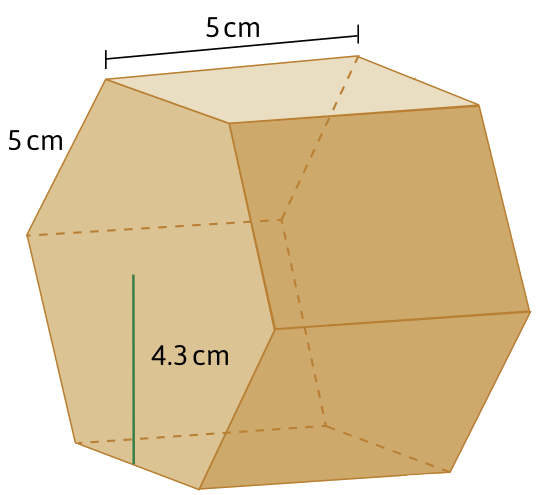
\includegraphics[width=.9\linewidth]{../images/20230319093449}
        \caption{}
        \label{fig:20230319093449}
    \end{figure}
\end{minipage}%
\begin{minipage}{0.65\linewidth}
    \begin{parts}
        \part Calcula su volumen

        \begin{solutionbox}{2cm}
            \[V=A_b h=\left(\dfrac{6\times 5 \text{ cm}\times 4.3 \text{ cm}}{2}\right)5 \text{ cm}=322.5 \text{ cm}^3
            \]
        \end{solutionbox}
        \part Otra caja de dulces tiene la misma forma, pero cada dimensión es el doble de las dimensiones de la otra caja. ¿Cuál será el volumen de esta segunda caja?

        \begin{solutionbox}{2.5cm}
            El volumen de una caja con el doble de dimensiones, sería:
            \[
                V=A_b h=\left(\dfrac{6\times 10 \text{ cm}\times 8 \text{ cm}}{2}\right)10 \text{ cm}=2580 \text{ cm}^3
            \]
        \end{solutionbox}
        \part ¿Cuántas veces es más grande el volumen de la caja mayor que la primera caja?

        \begin{solutionbox}{2.5cm}
            \[\dfrac{2 580 \text{ cm}^3}{322.5 \text{cm}^3}=8\]
            La caja con el doble de dimensiones es 8 veces mayor que la primera.
        \end{solutionbox}
    \end{parts}

\end{minipage}



